\documentclass[conference,compsoc]{IEEEtran}



% *** CITATION PACKAGES ***
%
\ifCLASSOPTIONcompsoc
  % IEEE Computer Society needs nocompress option
  % requires cite.sty v4.0 or later (November 2003)
  \usepackage[nocompress]{cite}
\else
  % normal IEEE
  \usepackage{cite}
\fi


% *** GRAPHICS RELATED PACKAGES ***
%
\ifCLASSINFOpdf
  % \usepackage[pdftex]{graphicx}
  % declare the path(s) where your graphic files are
  % \graphicspath{{../pdf/}{../jpeg/}}
  % and their extensions so you won't have to specify these with
  % every instance of \includegraphics
  % \DeclareGraphicsExtensions{.pdf,.jpeg,.png}
\else
  % or other class option (dvipsone, dvipdf, if not using dvips). graphicx
  % will default to the driver specified in the system graphics.cfg if no
  % driver is specified.
  % \usepackage[dvips]{graphicx}
  % declare the path(s) where your graphic files are
  % \graphicspath{{../eps/}}
  % and their extensions so you won't have to specify these with
  % every instance of \includegraphics
  % \DeclareGraphicsExtensions{.eps}
\fi



\usepackage{tikz}
\usepackage{graphicx}
\usetikzlibrary{shapes.geometric, arrows}
\tikzstyle{line}=[draw] % here
% correct bad hyphenation here
\hyphenation{op-tical net-works semi-conduc-tor}


\begin{document}
%
% paper title
\title{CSE 591 - Introduction to Deep Learning\\Mini Project 5}


% author names and affiliations
% use a multiple column layout for up to three different
% affiliations
\author{\IEEEauthorblockN{Bijan Fakhri}
\IEEEauthorblockA{School of Computing, Informatics and\\Decision Systems Engineering\\
Arizona State University\\
Tempe, Arizona 85044\\
Email: bfakhri@asu.edu}}

% make the title area
\maketitle

% As a general rule, do not put math, special symbols or citations
% in the abstract
\begin{abstract}
Comparing the filters after training a convolutional neural network (CNN) on several different datasets, it becomes evident that there exists some level of redundancy between the filters trained using different datasets. Because of this, we can devise that similar features exists in both datasets. This phenomena is called dataset generality. The purpose of this project is to measure this phenomena. 
\end{abstract}



\IEEEpeerreviewmaketitle



\section{Introduction}
% no \IEEEPARstart
Dataset generality can be leveraged to pretrain CNNs to save time training on new datasets. The usefulness of a dataset for such a task is, of course, related to the generality of the dataset. Relative dataset generality can be measured, as explained in \cite{DBLP:journals/corr/VenkatesanGL16}. The notation 
\begin{equation}
\Psi(D_j|r)
\end{equation}
describes the performance of a network trained on dataset $D_j$ and initialized with random weights. 


 


\section{Methodology}
To measure the generalities, we prejudiced a network using one dataset, and retrained solely the softmax layer on other another dataset

\section{Results}

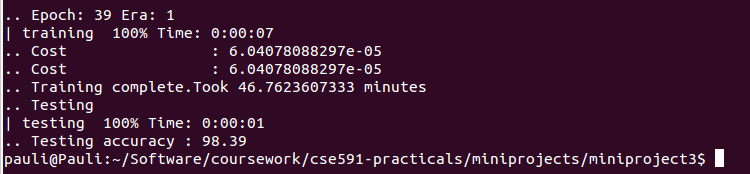
\includegraphics[scale=0.5]{orig}
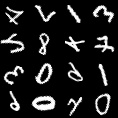
\includegraphics[scale=0.5]{rot}
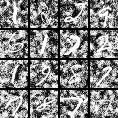
\includegraphics[scale=0.5]{noisy}
\section{Conclusion}
%
Reiterate meaning of results (quickly)

\nocite{*}
\bibliography{ragav}
%\bibliographystyle{IEEE}
\bibliographystyle{IEEEtran}

%\begin{thebibliography}{1}


%\bibitem{}
%REDO THIS 

%\bibitem{}
%H.~Kopka and P.~W. Daly, \emph{A Guide to \LaTeX}, 3rd~ed.\hskip 1em plus
%  0.5em minus 0.4em\relax Harlow, England: Addison-Wesley, 1999.
  


%\end{thebibliography}

% that's all folks
\end{document}


